% !TEX TS–program = pdflatexmk
\documentclass[12pt]{dmsthesis}
% Master master file for the NJIT DMS Dissertation / Thesis template.

% ----------------------------------------------------------------------
% Package Imports and Macros
% ----------------------------------------------------------------------
% !TeX root = main.tex

% Table and alignment packages
\usepackage{tabularx}
\usepackage{booktabs}
\usepackage{array}

% Math packages
\usepackage{amsmath,amsfonts,amssymb,amsthm,mathtools}

% Graphics and subfigures
\usepackage{graphicx}
\usepackage{subcaption}

% URL breaking for references and tables
\usepackage{xurl}

% Quotations
\usepackage{csquotes}
\MakeOuterQuote{"}

%% Bibliography (BibLaTeX with Biber backend)
\usepackage[backend=biber,doi=false,url=false,defernums=true,sortcites=true]{biblatex}

\defbibheading{subbibliography}[\refname]{%
	{\normalfont\large\bfseries}%
}

\addbibresource{references.bib}
% !TEX root = main.tex
% MACROS AND THEOREM ENVIRONMENTS (included via % !TEX root = main.tex
% MACROS AND THEOREM ENVIRONMENTS (included via % !TEX root = main.tex
% MACROS AND THEOREM ENVIRONMENTS (included via \input{macros} in main.tex)
%
% Define your own notation here with \newcommand, so each symbol is typed the
% same way everywhere and can be changed in one place. Add new theorem-like
% environments here too; they share one counter and are numbered by chapter
% (Theorem 2.1, Lemma 2.2, ...).

% Mathematical blackboard bold shortcuts
\newcommand{\CC}{\mathbb{C}}
\newcommand{\RR}{\mathbb{R}}
\newcommand{\ZZ}{\mathbb{Z}}
\newcommand{\NN}{\mathbb{N}}
\newcommand{\QQ}{\mathbb{Q}}

% Trademark sign after a brand name: MATLAB\trademark
\newcommand{\trademark}{\textsuperscript{\texttrademark}}

% Standard BibTeX logo
\DeclareRobustCommand{\BibTeX}{%
  {\normalfont B\kern-.05em{\scshape i\kern-.025em b}\kern-.08em \TeX}%
}

% Standard Theorem Environments (via amsthm)
\theoremstyle{plain}
\newtheorem{theorem}{Theorem}[chapter]
\newtheorem{lemma}[theorem]{Lemma}
\newtheorem{proposition}[theorem]{Proposition}
\newtheorem{corollary}[theorem]{Corollary}

\theoremstyle{definition}
\newtheorem{definition}[theorem]{Definition}
\newtheorem{example}[theorem]{Example}

\theoremstyle{remark}
\newtheorem{remark}[theorem]{Remark}
 in main.tex)
%
% Define your own notation here with \newcommand, so each symbol is typed the
% same way everywhere and can be changed in one place. Add new theorem-like
% environments here too; they share one counter and are numbered by chapter
% (Theorem 2.1, Lemma 2.2, ...).

% Mathematical blackboard bold shortcuts
\newcommand{\CC}{\mathbb{C}}
\newcommand{\RR}{\mathbb{R}}
\newcommand{\ZZ}{\mathbb{Z}}
\newcommand{\NN}{\mathbb{N}}
\newcommand{\QQ}{\mathbb{Q}}

% Trademark sign after a brand name: MATLAB\trademark
\newcommand{\trademark}{\textsuperscript{\texttrademark}}

% Standard BibTeX logo
\DeclareRobustCommand{\BibTeX}{%
  {\normalfont B\kern-.05em{\scshape i\kern-.025em b}\kern-.08em \TeX}%
}

% Standard Theorem Environments (via amsthm)
\theoremstyle{plain}
\newtheorem{theorem}{Theorem}[chapter]
\newtheorem{lemma}[theorem]{Lemma}
\newtheorem{proposition}[theorem]{Proposition}
\newtheorem{corollary}[theorem]{Corollary}

\theoremstyle{definition}
\newtheorem{definition}[theorem]{Definition}
\newtheorem{example}[theorem]{Example}

\theoremstyle{remark}
\newtheorem{remark}[theorem]{Remark}
 in main.tex)
%
% Define your own notation here with \newcommand, so each symbol is typed the
% same way everywhere and can be changed in one place. Add new theorem-like
% environments here too; they share one counter and are numbered by chapter
% (Theorem 2.1, Lemma 2.2, ...).

% Mathematical blackboard bold shortcuts
\newcommand{\CC}{\mathbb{C}}
\newcommand{\RR}{\mathbb{R}}
\newcommand{\ZZ}{\mathbb{Z}}
\newcommand{\NN}{\mathbb{N}}
\newcommand{\QQ}{\mathbb{Q}}

% Trademark sign after a brand name: MATLAB\trademark
\newcommand{\trademark}{\textsuperscript{\texttrademark}}

% Standard BibTeX logo
\DeclareRobustCommand{\BibTeX}{%
  {\normalfont B\kern-.05em{\scshape i\kern-.025em b}\kern-.08em \TeX}%
}

% Standard Theorem Environments (via amsthm)
\theoremstyle{plain}
\newtheorem{theorem}{Theorem}[chapter]
\newtheorem{lemma}[theorem]{Lemma}
\newtheorem{proposition}[theorem]{Proposition}
\newtheorem{corollary}[theorem]{Corollary}

\theoremstyle{definition}
\newtheorem{definition}[theorem]{Definition}
\newtheorem{example}[theorem]{Example}

\theoremstyle{remark}
\newtheorem{remark}[theorem]{Remark}


% Graphics directory
\graphicspath{{Graphics/}}

\begin{document}

%%%%%%%%%%%%%%%%%%%%%%%%%%%%%%%%%%%%%%%%%%%%%%%%%%%%%%%%%%%%%%
%  Front Matter Initialization Pages:
%       ABSTRACT PAGE       (abstract.tex)
%       TITLE PAGE          (created by class file)
%       COPYRIGHT PAGE      (created by class file)
%       APPROVAL PAGE       (approval.tex)
%       BIOGRAPHY PAGE      (biography.tex)
%       DEDICATION PAGE     (dedication.tex, optional)
%       ACKNOWLEDGMENT PAGE (acknowledgment.tex)
%%%%%%%%%%%%%%%%%%%%%%%%%%%%%%%%%%%%%%%%%%%%%%%%%%%%%%%%%%%%%%

\abstract{\noindent
% Start typing your abstract below this line


% Delete everything below
\noindent

This document contains instructions for preparing an NJIT dissertation and is, itself, a properly formatted demonstration of a dissertation. This is packaged as a set of files. You put different things in different files. We'll tell you what goes in where. The goal is to have all the formatting taken care of and allow you to concentrate on writing a great dissertation. Still, based on your judgment and the GSO's watchful eye, you'll likely make changes. We encourage you to contribute changes and make pull requests on GitHub, in order that future students may benefit from your experience.
}
% Note:  Advisor's title and Committee member's title must be checked against
% graduate catalog (example is given after the general format).

%The "\" after "Dr." prevents inter-sentence spacing
\advisor{Dr.\ Courtney Vandersloot} 
	    {Professor of Basketball, NJIT} 

\member{Dr.\ Betnijah Laney-Hamilton}
       {Associate Professor of Basketball, NJIT}

\member{Dr.\ Jonquel Jones}
       {Associate Professor of Basketball, NJIT}
	
\member{Dr.\ Breanna ``Stewie'' Stewart}
       {Associate Professor of Basketball, NJIT}
	
\member{Dr.\ Sabrina Ionescu }
       {Assistant Professor of Computer and Information Science, Some Other University}

% !TEX root = main.tex
% TITLE-PAGE AND BIOGRAPHICAL SKETCH INFORMATION
% (included via % !TEX root = main.tex
% TITLE-PAGE AND BIOGRAPHICAL SKETCH INFORMATION
% (included via % !TEX root = main.tex
% TITLE-PAGE AND BIOGRAPHICAL SKETCH INFORMATION
% (included via \input{biography} in main.tex)
%
% Everything here is set ONCE and reused on the abstract, title, copyright,
% approval and biography pages, so the pages cannot disagree.
%
% \title           Type it in normal capitalization; the class sets it in
%                  capitals where the GSO requires.
% \author          Your name exactly as it should appear on the diploma.
% \graduationdate  Month (May, August or December) and year you GRADUATE,
%                  not the date you defend.
% \thisdegree      Full name of the degree you are receiving.
% \degreeearned    One line per degree earned, MOST RECENT FIRST, starting
%                  with the degree you are receiving now:
%                  \degreeearned{Degree name}{University, City, State, Year}.
%                  Use the exact degree title from your transcript.
% \degreelevel     Optional. Overrides the "Degree:" line of the sketch,
%                  which defaults to "Doctor of Philosophy" (or "Master of
%                  Science" with the thesis class option).
%
% For a master's thesis, use \documentclass[12pt,thesis]{njit_thesis} in
% main.tex: the title page says "A Thesis" and the copyright page is blank.
%
% Presentations and publications are listed automatically from
% references.bib, newest first: add  keywords = {me}  to each of your own
% entries. Papers in preparation, submitted or under review may be included.

\title{Title of your dissertation}

\author{Your Name}

\major{Your Major}

% Month (May, August or December) and year you GRADUATE
\graduationdate{May}{2026}

\thisdegree{Doctor of Philosophy in Your Major}
\department{Department of Your Department}

%% Uncomment one of the following two institutes
%% For departments/degrees at NJIT
\institute{New Jersey Institute of Technology}
%% For departments/degrees joint with RU-Newark (including the math department)
% \institute{New Jersey Institute of Technology and \par Rutgers, The State University of New Jersey---Newark}

% List degrees with most recent first, starting with the degree you are
% about to receive.
\degreeearned{Doctor of Philosophy in Your Major}{New Jersey Institute of Technology, Newark, NJ, 2026}

\degreeearned{Bachelor of Science in Your Major}{Your College, City, ST, 2020}

% If you don't have any publications uncomment below
%\renewcommand{\printmypublications}{}
 in main.tex)
%
% Everything here is set ONCE and reused on the abstract, title, copyright,
% approval and biography pages, so the pages cannot disagree.
%
% \title           Type it in normal capitalization; the class sets it in
%                  capitals where the GSO requires.
% \author          Your name exactly as it should appear on the diploma.
% \graduationdate  Month (May, August or December) and year you GRADUATE,
%                  not the date you defend.
% \thisdegree      Full name of the degree you are receiving.
% \degreeearned    One line per degree earned, MOST RECENT FIRST, starting
%                  with the degree you are receiving now:
%                  \degreeearned{Degree name}{University, City, State, Year}.
%                  Use the exact degree title from your transcript.
% \degreelevel     Optional. Overrides the "Degree:" line of the sketch,
%                  which defaults to "Doctor of Philosophy" (or "Master of
%                  Science" with the thesis class option).
%
% For a master's thesis, use \documentclass[12pt,thesis]{njit_thesis} in
% main.tex: the title page says "A Thesis" and the copyright page is blank.
%
% Presentations and publications are listed automatically from
% references.bib, newest first: add  keywords = {me}  to each of your own
% entries. Papers in preparation, submitted or under review may be included.

\title{Title of your dissertation}

\author{Your Name}

\major{Your Major}

% Month (May, August or December) and year you GRADUATE
\graduationdate{May}{2026}

\thisdegree{Doctor of Philosophy in Your Major}
\department{Department of Your Department}

%% Uncomment one of the following two institutes
%% For departments/degrees at NJIT
\institute{New Jersey Institute of Technology}
%% For departments/degrees joint with RU-Newark (including the math department)
% \institute{New Jersey Institute of Technology and \par Rutgers, The State University of New Jersey---Newark}

% List degrees with most recent first, starting with the degree you are
% about to receive.
\degreeearned{Doctor of Philosophy in Your Major}{New Jersey Institute of Technology, Newark, NJ, 2026}

\degreeearned{Bachelor of Science in Your Major}{Your College, City, ST, 2020}

% If you don't have any publications uncomment below
%\renewcommand{\printmypublications}{}
 in main.tex)
%
% Everything here is set ONCE and reused on the abstract, title, copyright,
% approval and biography pages, so the pages cannot disagree.
%
% \title           Type it in normal capitalization; the class sets it in
%                  capitals where the GSO requires.
% \author          Your name exactly as it should appear on the diploma.
% \graduationdate  Month (May, August or December) and year you GRADUATE,
%                  not the date you defend.
% \thisdegree      Full name of the degree you are receiving.
% \degreeearned    One line per degree earned, MOST RECENT FIRST, starting
%                  with the degree you are receiving now:
%                  \degreeearned{Degree name}{University, City, State, Year}.
%                  Use the exact degree title from your transcript.
% \degreelevel     Optional. Overrides the "Degree:" line of the sketch,
%                  which defaults to "Doctor of Philosophy" (or "Master of
%                  Science" with the thesis class option).
%
% For a master's thesis, use \documentclass[12pt,thesis]{njit_thesis} in
% main.tex: the title page says "A Thesis" and the copyright page is blank.
%
% Presentations and publications are listed automatically from
% references.bib, newest first: add  keywords = {me}  to each of your own
% entries. Papers in preparation, submitted or under review may be included.

\title{Title of your dissertation}

\author{Your Name}

\major{Your Major}

% Month (May, August or December) and year you GRADUATE
\graduationdate{May}{2026}

\thisdegree{Doctor of Philosophy in Your Major}
\department{Department of Your Department}

%% Uncomment one of the following two institutes
%% For departments/degrees at NJIT
\institute{New Jersey Institute of Technology}
%% For departments/degrees joint with RU-Newark (including the math department)
% \institute{New Jersey Institute of Technology and \par Rutgers, The State University of New Jersey---Newark}

% List degrees with most recent first, starting with the degree you are
% about to receive.
\degreeearned{Doctor of Philosophy in Your Major}{New Jersey Institute of Technology, Newark, NJ, 2026}

\degreeearned{Bachelor of Science in Your Major}{Your College, City, ST, 2020}

% If you don't have any publications uncomment below
%\renewcommand{\printmypublications}{}

\dedication{% !TEX root = main.tex
% DEDICATION (optional; included via \dedication{% !TEX root = main.tex
% DEDICATION (optional; included via \dedication{% !TEX root = main.tex
% DEDICATION (optional; included via \dedication{\input{dedication}} in main.tex)
%
% A short dedication or quotation, set single-spaced in a centered block.
% Check the spelling of names and keep person and tense consistent (GSO).
% To omit the page, comment out the \dedication line in main.tex.
% Words left out of a quotation are marked with an ellipsis, typed \ldots;
% between two full sentences the first keeps its period (Chicago style).

\emph{Power of concentration is a very valuable quality, which few people acquire except through education. \ldots{} To be able to concentrate on the same matter for a considerable time is essential to difficult achievement, and even to the understanding of any complicated or abstruse subject.}

\begin{flushright}
Bertrand Russell, \emph{On Education} (1926)
\end{flushright}
} in main.tex)
%
% A short dedication or quotation, set single-spaced in a centered block.
% Check the spelling of names and keep person and tense consistent (GSO).
% To omit the page, comment out the \dedication line in main.tex.
% Words left out of a quotation are marked with an ellipsis, typed \ldots;
% between two full sentences the first keeps its period (Chicago style).

\emph{Power of concentration is a very valuable quality, which few people acquire except through education. \ldots{} To be able to concentrate on the same matter for a considerable time is essential to difficult achievement, and even to the understanding of any complicated or abstruse subject.}

\begin{flushright}
Bertrand Russell, \emph{On Education} (1926)
\end{flushright}
} in main.tex)
%
% A short dedication or quotation, set single-spaced in a centered block.
% Check the spelling of names and keep person and tense consistent (GSO).
% To omit the page, comment out the \dedication line in main.tex.
% Words left out of a quotation are marked with an ellipsis, typed \ldots;
% between two full sentences the first keeps its period (Chicago style).

\emph{Power of concentration is a very valuable quality, which few people acquire except through education. \ldots{} To be able to concentrate on the same matter for a considerable time is essential to difficult achievement, and even to the understanding of any complicated or abstruse subject.}

\begin{flushright}
Bertrand Russell, \emph{On Education} (1926)
\end{flushright}
}
\acknowledgment{% !TEX root = main.tex
% ACKNOWLEDGMENTS (included via \acknowledgment{% !TEX root = main.tex
% ACKNOWLEDGMENTS (included via \acknowledgment{% !TEX root = main.tex
% ACKNOWLEDGMENTS (included via \acknowledgment{\input{acknowledgment}} in main.tex)
%
% Write ordinary paragraphs; the class prints the heading and double-spaces
% the text. Do not use \noindent.
%
% GSO order: your ADVISOR first, then your COMMITTEE, then other
% contributors and peers, family, funding sources, and technical support.
% Acknowledge each grant by agency and grant number.

I thank my advisor, Dr.\ Advisor Name, for their guidance. Lorem ipsum dolor sit amet, consectetur adipiscing elit, sed do eiusmod tempor incididunt ut labore et dolore magna aliqua.

I thank my committee members, Drs.\ Member One, Member Two, Member Three, and Member Four. Ut enim ad minim veniam, quis nostrud exercitation ullamco laboris nisi ut aliquip ex ea commodo consequat.
} in main.tex)
%
% Write ordinary paragraphs; the class prints the heading and double-spaces
% the text. Do not use \noindent.
%
% GSO order: your ADVISOR first, then your COMMITTEE, then other
% contributors and peers, family, funding sources, and technical support.
% Acknowledge each grant by agency and grant number.

I thank my advisor, Dr.\ Advisor Name, for their guidance. Lorem ipsum dolor sit amet, consectetur adipiscing elit, sed do eiusmod tempor incididunt ut labore et dolore magna aliqua.

I thank my committee members, Drs.\ Member One, Member Two, Member Three, and Member Four. Ut enim ad minim veniam, quis nostrud exercitation ullamco laboris nisi ut aliquip ex ea commodo consequat.
} in main.tex)
%
% Write ordinary paragraphs; the class prints the heading and double-spaces
% the text. Do not use \noindent.
%
% GSO order: your ADVISOR first, then your COMMITTEE, then other
% contributors and peers, family, funding sources, and technical support.
% Acknowledge each grant by agency and grant number.

I thank my advisor, Dr.\ Advisor Name, for their guidance. Lorem ipsum dolor sit amet, consectetur adipiscing elit, sed do eiusmod tempor incididunt ut labore et dolore magna aliqua.

I thank my committee members, Drs.\ Member One, Member Two, Member Three, and Member Four. Ut enim ad minim veniam, quis nostrud exercitation ullamco laboris nisi ut aliquip ex ea commodo consequat.
}

% Optional preliminary lists data
\symbols{% !TEX root = main.tex
% List of Symbols (included via \symbols{% !TEX root = main.tex
% List of Symbols (included via \symbols{% !TEX root = main.tex
% List of Symbols (included via \symbols{\input{listofsymbols}} in main.tex)
%
% A two-column table: the symbol, then its description. Start each
% description with a capital letter and write it in sentence case (GSO).
% Organize the list by category or function, alphabetically by name, or by
% frequency of use (GSO). Alphabetical order follows the characters
% themselves, so * comes after &. The sample is organized by category.
% The table continues across pages automatically. To widen the symbol
% column, give a width: \begin{symboltable}[1.5in]

\begin{symboltable}
% Number systems
\sym{$\ZZ$}{The ring of integers}
\sym{$\RR$}{The field of real numbers}
\sym{$\CC$}{The field of complex numbers}
% Spaces and groups
\sym{$H^1(\RR)$}{The Sobolev space of functions over $\RR$ that are square-integrable and whose weak first derivative is square-integrable}
\sym{$\mathrm{GL}_2(\RR)$}{The general linear group of real invertible $2\times 2$ matrices}
% Physical quantities
\sym{$c$}{Speed of light in vacuum ($c \approx 3 \times 10^8\text{ m/s}$)}
\sym{$E$}{Energy of a physical system}
\sym{$m$}{Mass of a physical body}
% Other notation
\sym{$\%$}{Percentage sign}
\end{symboltable}
} in main.tex)
%
% A two-column table: the symbol, then its description. Start each
% description with a capital letter and write it in sentence case (GSO).
% Organize the list by category or function, alphabetically by name, or by
% frequency of use (GSO). Alphabetical order follows the characters
% themselves, so * comes after &. The sample is organized by category.
% The table continues across pages automatically. To widen the symbol
% column, give a width: \begin{symboltable}[1.5in]

\begin{symboltable}
% Number systems
\sym{$\ZZ$}{The ring of integers}
\sym{$\RR$}{The field of real numbers}
\sym{$\CC$}{The field of complex numbers}
% Spaces and groups
\sym{$H^1(\RR)$}{The Sobolev space of functions over $\RR$ that are square-integrable and whose weak first derivative is square-integrable}
\sym{$\mathrm{GL}_2(\RR)$}{The general linear group of real invertible $2\times 2$ matrices}
% Physical quantities
\sym{$c$}{Speed of light in vacuum ($c \approx 3 \times 10^8\text{ m/s}$)}
\sym{$E$}{Energy of a physical system}
\sym{$m$}{Mass of a physical body}
% Other notation
\sym{$\%$}{Percentage sign}
\end{symboltable}
} in main.tex)
%
% A two-column table: the symbol, then its description. Start each
% description with a capital letter and write it in sentence case (GSO).
% Organize the list by category or function, alphabetically by name, or by
% frequency of use (GSO). Alphabetical order follows the characters
% themselves, so * comes after &. The sample is organized by category.
% The table continues across pages automatically. To widen the symbol
% column, give a width: \begin{symboltable}[1.5in]

\begin{symboltable}
% Number systems
\sym{$\ZZ$}{The ring of integers}
\sym{$\RR$}{The field of real numbers}
\sym{$\CC$}{The field of complex numbers}
% Spaces and groups
\sym{$H^1(\RR)$}{The Sobolev space of functions over $\RR$ that are square-integrable and whose weak first derivative is square-integrable}
\sym{$\mathrm{GL}_2(\RR)$}{The general linear group of real invertible $2\times 2$ matrices}
% Physical quantities
\sym{$c$}{Speed of light in vacuum ($c \approx 3 \times 10^8\text{ m/s}$)}
\sym{$E$}{Energy of a physical system}
\sym{$m$}{Mass of a physical body}
% Other notation
\sym{$\%$}{Percentage sign}
\end{symboltable}
}
\glossaryofterms{% !TEX root = main.tex
% Glossary of Terms (included via \glossaryofterms{% !TEX root = main.tex
% Glossary of Terms (included via \glossaryofterms{% !TEX root = main.tex
% Glossary of Terms (included via \glossaryofterms{\input{listofdefinitions}} in main.tex)
%
% A two-column table: the term, then its definition. List terms in
% alphabetical order. Start each definition with a capital letter and write
% it in sentence case; capitalize only acronyms and proper names (GSO).
% The table continues across pages automatically. To change the width of
% the term column, give a width: \begin{glossarytable}[2in]
%
% Commands cannot be shown with \verb here, because this file is passed as an
% argument; write \texttt{\textbackslash{}cite\{key\}} instead.

\begin{glossarytable}
\term{Argument}{Input given to a command in braces, as in \texttt{\textbackslash{}section\{Title\}}. Optional arguments go in square brackets, as in \texttt{\textbackslash{}includegraphics[width=3in]\{file\}}.}
\term{Auxiliary file}{A file such as \texttt{main.aux} or \texttt{main.toc} that \LaTeX\ writes during one run and reads on the next to resolve cross-references and lists. Deleting these files is a safe first step when a build behaves strangely.}
\term{Biber}{The program that reads \texttt{references.bib} and sorts and formats the bibliography for \texttt{biblatex}. It runs between \LaTeX\ runs.}
\term{\texttt{biblatex}}{The package that formats citations and the bibliography. The citation style is chosen once, in \texttt{packages.tex}.}
\term{\BibTeX\ entry}{One record in a \texttt{.bib} file, such as \texttt{@article\{key, ...\}}. The key is the name used in \texttt{\textbackslash{}cite\{key\}}.}
\term{Class file}{A file ending in \texttt{.cls} that defines a document's overall layout. This template's class, \texttt{njit\_thesis.cls}, implements the NJIT formatting rules.}
\term{Command}{An instruction that begins with a backslash, such as \texttt{\textbackslash{}chapter} or \texttt{\textbackslash{}cite}.}
\term{Comment}{Text after a \texttt{\%} sign on a line. \LaTeX\ ignores it, so comments are useful for notes and for temporarily removing material.}
\term{Cross-reference}{A reference to a numbered item, made with \texttt{\textbackslash{}label} and \texttt{\textbackslash{}ref} (or \texttt{\textbackslash{}eqref} for equations). Numbers update automatically when material moves.}
\term{Environment}{A block of material between \texttt{\textbackslash{}begin\{name\}} and \texttt{\textbackslash{}end\{name\}}, such as \texttt{figure}, \texttt{table}, or \texttt{equation}.}
\term{Float}{A figure or table that \LaTeX\ may move to a nearby page to avoid large gaps. Always refer to floats by number, not as ``the figure below.''}
\term{Label}{A name attached to a numbered item with \texttt{\textbackslash{}label\{name\}}, so it can be referred to with \texttt{\textbackslash{}ref\{name\}}. Prefixes such as \texttt{fig:} or \texttt{eq:} keep labels organized.}
\term{\texttt{latexmk}}{A program that runs \LaTeX\ and Biber as many times as needed to produce a complete document. Running \texttt{latexmk -pdf main.tex} builds this thesis.}
\term{Log file}{The file \texttt{main.log}, which records every warning and error from a run. Check it for undefined references and overfull boxes before submitting.}
\term{Macro}{A command you define yourself with \texttt{\textbackslash{}newcommand}, usually in \texttt{macros.tex}, to keep notation consistent and save typing.}
\term{Overfull box}{A warning that a line or object is too wide and sticks into the margin. The GSO checks margins, so fix these by rewording, adding a hyphenation point, or resizing the object.}
\term{Overleaf}{A website for editing and compiling \LaTeX\ documents in a browser, with no local installation.}
\term{Package}{A file loaded with \texttt{\textbackslash{}usepackage} that adds features, such as \texttt{amsmath} for mathematics or \texttt{graphicx} for images. This template loads its packages in \texttt{packages.tex}.}
\term{Preamble}{Everything in \texttt{main.tex} before \texttt{\textbackslash{}begin\{document\}}, where the class, packages, and macros are loaded.}
\term{Undefined reference}{A \texttt{\textbackslash{}ref} or \texttt{\textbackslash{}cite} that \LaTeX\ cannot resolve, shown as ``??'' in the PDF. It usually means a misspelled label or citation key, or that the document needs another run.}
\end{glossarytable}
} in main.tex)
%
% A two-column table: the term, then its definition. List terms in
% alphabetical order. Start each definition with a capital letter and write
% it in sentence case; capitalize only acronyms and proper names (GSO).
% The table continues across pages automatically. To change the width of
% the term column, give a width: \begin{glossarytable}[2in]
%
% Commands cannot be shown with \verb here, because this file is passed as an
% argument; write \texttt{\textbackslash{}cite\{key\}} instead.

\begin{glossarytable}
\term{Argument}{Input given to a command in braces, as in \texttt{\textbackslash{}section\{Title\}}. Optional arguments go in square brackets, as in \texttt{\textbackslash{}includegraphics[width=3in]\{file\}}.}
\term{Auxiliary file}{A file such as \texttt{main.aux} or \texttt{main.toc} that \LaTeX\ writes during one run and reads on the next to resolve cross-references and lists. Deleting these files is a safe first step when a build behaves strangely.}
\term{Biber}{The program that reads \texttt{references.bib} and sorts and formats the bibliography for \texttt{biblatex}. It runs between \LaTeX\ runs.}
\term{\texttt{biblatex}}{The package that formats citations and the bibliography. The citation style is chosen once, in \texttt{packages.tex}.}
\term{\BibTeX\ entry}{One record in a \texttt{.bib} file, such as \texttt{@article\{key, ...\}}. The key is the name used in \texttt{\textbackslash{}cite\{key\}}.}
\term{Class file}{A file ending in \texttt{.cls} that defines a document's overall layout. This template's class, \texttt{njit\_thesis.cls}, implements the NJIT formatting rules.}
\term{Command}{An instruction that begins with a backslash, such as \texttt{\textbackslash{}chapter} or \texttt{\textbackslash{}cite}.}
\term{Comment}{Text after a \texttt{\%} sign on a line. \LaTeX\ ignores it, so comments are useful for notes and for temporarily removing material.}
\term{Cross-reference}{A reference to a numbered item, made with \texttt{\textbackslash{}label} and \texttt{\textbackslash{}ref} (or \texttt{\textbackslash{}eqref} for equations). Numbers update automatically when material moves.}
\term{Environment}{A block of material between \texttt{\textbackslash{}begin\{name\}} and \texttt{\textbackslash{}end\{name\}}, such as \texttt{figure}, \texttt{table}, or \texttt{equation}.}
\term{Float}{A figure or table that \LaTeX\ may move to a nearby page to avoid large gaps. Always refer to floats by number, not as ``the figure below.''}
\term{Label}{A name attached to a numbered item with \texttt{\textbackslash{}label\{name\}}, so it can be referred to with \texttt{\textbackslash{}ref\{name\}}. Prefixes such as \texttt{fig:} or \texttt{eq:} keep labels organized.}
\term{\texttt{latexmk}}{A program that runs \LaTeX\ and Biber as many times as needed to produce a complete document. Running \texttt{latexmk -pdf main.tex} builds this thesis.}
\term{Log file}{The file \texttt{main.log}, which records every warning and error from a run. Check it for undefined references and overfull boxes before submitting.}
\term{Macro}{A command you define yourself with \texttt{\textbackslash{}newcommand}, usually in \texttt{macros.tex}, to keep notation consistent and save typing.}
\term{Overfull box}{A warning that a line or object is too wide and sticks into the margin. The GSO checks margins, so fix these by rewording, adding a hyphenation point, or resizing the object.}
\term{Overleaf}{A website for editing and compiling \LaTeX\ documents in a browser, with no local installation.}
\term{Package}{A file loaded with \texttt{\textbackslash{}usepackage} that adds features, such as \texttt{amsmath} for mathematics or \texttt{graphicx} for images. This template loads its packages in \texttt{packages.tex}.}
\term{Preamble}{Everything in \texttt{main.tex} before \texttt{\textbackslash{}begin\{document\}}, where the class, packages, and macros are loaded.}
\term{Undefined reference}{A \texttt{\textbackslash{}ref} or \texttt{\textbackslash{}cite} that \LaTeX\ cannot resolve, shown as ``??'' in the PDF. It usually means a misspelled label or citation key, or that the document needs another run.}
\end{glossarytable}
} in main.tex)
%
% A two-column table: the term, then its definition. List terms in
% alphabetical order. Start each definition with a capital letter and write
% it in sentence case; capitalize only acronyms and proper names (GSO).
% The table continues across pages automatically. To change the width of
% the term column, give a width: \begin{glossarytable}[2in]
%
% Commands cannot be shown with \verb here, because this file is passed as an
% argument; write \texttt{\textbackslash{}cite\{key\}} instead.

\begin{glossarytable}
\term{Argument}{Input given to a command in braces, as in \texttt{\textbackslash{}section\{Title\}}. Optional arguments go in square brackets, as in \texttt{\textbackslash{}includegraphics[width=3in]\{file\}}.}
\term{Auxiliary file}{A file such as \texttt{main.aux} or \texttt{main.toc} that \LaTeX\ writes during one run and reads on the next to resolve cross-references and lists. Deleting these files is a safe first step when a build behaves strangely.}
\term{Biber}{The program that reads \texttt{references.bib} and sorts and formats the bibliography for \texttt{biblatex}. It runs between \LaTeX\ runs.}
\term{\texttt{biblatex}}{The package that formats citations and the bibliography. The citation style is chosen once, in \texttt{packages.tex}.}
\term{\BibTeX\ entry}{One record in a \texttt{.bib} file, such as \texttt{@article\{key, ...\}}. The key is the name used in \texttt{\textbackslash{}cite\{key\}}.}
\term{Class file}{A file ending in \texttt{.cls} that defines a document's overall layout. This template's class, \texttt{njit\_thesis.cls}, implements the NJIT formatting rules.}
\term{Command}{An instruction that begins with a backslash, such as \texttt{\textbackslash{}chapter} or \texttt{\textbackslash{}cite}.}
\term{Comment}{Text after a \texttt{\%} sign on a line. \LaTeX\ ignores it, so comments are useful for notes and for temporarily removing material.}
\term{Cross-reference}{A reference to a numbered item, made with \texttt{\textbackslash{}label} and \texttt{\textbackslash{}ref} (or \texttt{\textbackslash{}eqref} for equations). Numbers update automatically when material moves.}
\term{Environment}{A block of material between \texttt{\textbackslash{}begin\{name\}} and \texttt{\textbackslash{}end\{name\}}, such as \texttt{figure}, \texttt{table}, or \texttt{equation}.}
\term{Float}{A figure or table that \LaTeX\ may move to a nearby page to avoid large gaps. Always refer to floats by number, not as ``the figure below.''}
\term{Label}{A name attached to a numbered item with \texttt{\textbackslash{}label\{name\}}, so it can be referred to with \texttt{\textbackslash{}ref\{name\}}. Prefixes such as \texttt{fig:} or \texttt{eq:} keep labels organized.}
\term{\texttt{latexmk}}{A program that runs \LaTeX\ and Biber as many times as needed to produce a complete document. Running \texttt{latexmk -pdf main.tex} builds this thesis.}
\term{Log file}{The file \texttt{main.log}, which records every warning and error from a run. Check it for undefined references and overfull boxes before submitting.}
\term{Macro}{A command you define yourself with \texttt{\textbackslash{}newcommand}, usually in \texttt{macros.tex}, to keep notation consistent and save typing.}
\term{Overfull box}{A warning that a line or object is too wide and sticks into the margin. The GSO checks margins, so fix these by rewording, adding a hyphenation point, or resizing the object.}
\term{Overleaf}{A website for editing and compiling \LaTeX\ documents in a browser, with no local installation.}
\term{Package}{A file loaded with \texttt{\textbackslash{}usepackage} that adds features, such as \texttt{amsmath} for mathematics or \texttt{graphicx} for images. This template loads its packages in \texttt{packages.tex}.}
\term{Preamble}{Everything in \texttt{main.tex} before \texttt{\textbackslash{}begin\{document\}}, where the class, packages, and macros are loaded.}
\term{Undefined reference}{A \texttt{\textbackslash{}ref} or \texttt{\textbackslash{}cite} that \LaTeX\ cannot resolve, shown as ``??'' in the PDF. It usually means a misspelled label or citation key, or that the document needs another run.}
\end{glossarytable}
}

% Generate all front matter pages in NJIT prescribed order
\initthesis

%%%%%%%%%%%%%%%%%%%%%%%%%%%%%%%%%%%%%%%%%%%%%%%%%%%%%%
%  Table of Contents and Preliminary Lists:
%       TABLE OF CONTENTS
%       LIST OF TABLES
%       LIST OF FIGURES
%       LIST OF SYMBOLS (optional)
%       GLOSSARY OF TERMS (optional)
%%%%%%%%%%%%%%%%%%%%%%%%%%%%%%%%%%%%%%%%%%%%%%%%%%%%%%
\tableofcontents
\listoftables
\listoffigures
\makelistofsymbols
\makeglossaryofterms

%%%%%%%%%%%%%%%%%%%%%%%%%%%%%%%%%%%%%%%%%%%%%%%%%%%%%%
%% START MAIN BODY OF THESIS
%% Arabic page numbering (1, 2, 3...) begins here
%%%%%%%%%%%%%%%%%%%%%%%%%%%%%%%%%%%%%%%%%%%%%%%%%%%%%%
\startbody

% Optional Preface (must appear immediately before Chapter 1)
% !TeX root = main.tex
\begin{preface}

This is a preface. It is optional and must come immediately before Chapter~1.

This sample document serves as both a user's guide and a comprehensive demonstration of the \texttt{dmsthesis.cls} \LaTeX\ class for dissertations and theses at the New Jersey Institute of Technology Department of Mathematical Sciences. Chapter~1 details the functional structure of the files that compose the dissertation and explains the university formatting requirements. Chapter~2 demonstrates formatting for mathematical content, theorems, definitions, figures, subfigures, standard and landscape tables, and the bibliography.

\end{preface}

% Dissertation Chapters
% !TeX root = main.tex
% Chapter 1: the parts of a dissertation, what the template handles, the
% files you edit, and how to compile.
%
% Each chapter lives in its own file, included from main.tex with \input.
% Start the file with \chapter{Title}; type the title in normal
% capitalization (the class sets it in capitals). Headings below it:
%   \section       level 2, Title Case
%   \subsection    level 3, sentence case
%   \subsubsection level 4, sentence case, run-in (the class adds the period)
%   \paragraph     level 5, sentence case, italic (the class adds the period)
% Every heading needs a title; an empty one stops the build with an error.

\chapter{Getting Started}
\label{ch:start}

A \LaTeX\ dissertation project is structured like a well-organized software codebase: split into modular functional units contained in separate files. This chapter lists the parts an NJIT dissertation must contain, in the order required by the New Jersey Institute of Technology Office of Graduate Studies (GSO), summarizes the formatting rules the template applies for you, explains which files you edit, and shows how to compile the project locally and on Overleaf. Chapter~\ref{ch:writing} covers writing the text, Chapter~\ref{ch:figtables} covers figures and tables, and Chapter~\ref{ch:references} covers references and the checks to make before you submit. Four appendices follow. Appendix~\ref{app:appendixA} explains what belongs in an appendix and how to set one up, Appendix~\ref{app:citestyles} collects guides and examples for the accepted citation styles, Appendix~\ref{app:packages} describes the packages the template loads, and Appendix~\ref{app:filetree} lists the template's files.

\section{The Parts of a Dissertation, in Order}

An NJIT dissertation consists of three primary divisions: the preliminary front matter, the main body (chapters and appendices), and the back matter (references). These components appear in the following strict order:

\begin{description}
\emergencystretch=2em
\item[Abstract] A concise summary of the research questions, methodology, and conclusions. By NJIT guidelines, this page is unnumbered and precedes the title page. Defined in \texttt{abstract.tex} and generated by \verb+\makeabstract+.

\item[Title Page] The formal title page declaring degree, department, joint institution (if applicable), and graduation month and year. This page is considered Roman numeral~i, but no number is displayed on the page. Generated automatically by \verb+\maketitle+ using metadata in \texttt{biography.tex}.

\item[Copyright Page] Declares the copyright holder and year. Unnumbered. Required only for doctoral dissertations; a master's thesis has a blank page in its place (GSO), which the \texttt{thesis} class option produces. Generated automatically by \verb+\makecopyright+.

\item[Approval Page] Contains the signature lines for the dissertation advisor (and co-advisor, if any) and committee members with their official academic titles as listed in the graduate catalog. Unnumbered. Configured in \texttt{approval.tex} and generated by \verb+\makeapproval+.

\item[Biographical Sketch] Displays academic background, degrees earned (in reverse chronological order), major field of study, and a listing of presentations and publications. Roman page numbering begins visibly here (typically on page~iv). Configured in \texttt{biography.tex} and generated by \verb+\makebiography+. The publication list is generated automatically via \BibTeX\ / \texttt{biblatex} using the keyword \texttt{me}.

\item[Dedication] (Optional) A brief personal dedication. Centered and formatted with single spacing. Configured in \texttt{dedication.tex} and generated by \verb+\makededication+.

\item[Acknowledgment] Formal recognition of academic guidance, committee assistance, grant funding and financial support, technical and administrative assistance, and personal gratitude. Configured in \texttt{acknowledgment.tex} and generated by \verb+\makeacknowledgment+.

\item[Table of Contents] Lists all chapters, sections, subsections, appendices, and post-TOC preliminary lists with leader dots connecting titles to page numbers. Generated automatically by \verb+\tableofcontents+.

\item[List of Tables] Generated automatically by \verb+\listoftables+. If your dissertation contains no tables, comment out this command in \texttt{main.tex}.

\item[List of Figures] Generated automatically by \verb+\listoffigures+. If your dissertation contains no figures, comment out this command in \texttt{main.tex}.

\item[List of Symbols] (Optional) Defines mathematical symbols and physical constants used throughout the text. Configured in \texttt{listofsymbols.tex} and generated by \verb+\makelistofsymbols+.

\item[Glossary of Terms] (Optional) An alphabetical list of definitions. Configured in \texttt{listofdefinitions.tex} and generated via \verb+\makeglossaryofterms+.


\item[Main Body] The dissertation chapters, beginning with Arabic page number~1 at \verb+\startbody+. Each chapter is housed in its own file (e.g., \texttt{chapter1.tex}, \texttt{chapter2.tex}). Page numbers are centered at the bottom of every page in bold (GSO).

\item[Appendices] Supplementary mathematical proofs, data tables, or algorithm listings. NJIT enforces a strict rule: if there is only a \textbf{single appendix}, it must be labeled \textbf{APPENDIX} (without a letter like "A"). If there are \textbf{multiple appendices}, they must be numbered \textbf{APPENDIX A}, \textbf{APPENDIX B}, etc. This template fully automates both cases; Appendix~\ref{app:appendixA} explains how, and what material belongs in an appendix.

\item[References] The bibliography, styled consistently and sorted according to the field's standard conventions. Generated from \texttt{references.bib} via \texttt{biblatex} and \texttt{biber}.
\end{description}

\section{What the Template Does for You}
\label{sec:template-does}

The class file applies most of the GSO's formatting rules automatically. Table~\ref{table:gso_rules} lists the main rules and shows which ones the template takes care of and which are up to you.

% !TeX root = main.tex
% Sample table, kept in its own file and included from chapter2.tex with
% % !TeX root = main.tex
% Sample table, kept in its own file and included from chapter2.tex with
% \input{table}. Separate files are optional but handy for large tables or
% tables generated by a script.
%
% GSO rules (the class handles the layout):
% - The title (\caption) goes ABOVE the table, in title case, with no final
%   period. It appears word for word in the List of Tables.
% - Tables are numbered by chapter (Table 2.1).
% - Table text is single-spaced; a small table must not split across pages.
% Refer to every table in the text with \ref{label}.

\begin{table}[htbp]
\centering
\caption{Major Differences Between Neural Networks and Cell Signaling Networks}
\label{table:NN_DIFF}

\begin{tabularx}{\linewidth}{|c|p{0.18\linewidth}|X|X|}
\hline
\textbf{Item} & \textbf{Salient Feature} & \textbf{Neural Networks} & \textbf{Cell Signaling Networks} \\
\hline
(i) & Nodes & All nodes typically identical & Nodes are not all equivalent in performance \\
\hline
(ii) & Structure & Typically layered with feed-forward connections only & Regulatory signals often give rise to feedback connections resulting in cycles \\
\hline
(iii) & Connectivity & Highly connected & More sparsely connected \\
\hline
(iv) & Learning Rule & Connectivity altered to perform a single function (e.g., via a back-propagation algorithm) & Cells must be able to respond to multiple stimuli effectively; changes typically occur via evolutionary processes \\
\hline
\end{tabularx}
\end{table}
. Separate files are optional but handy for large tables or
% tables generated by a script.
%
% GSO rules (the class handles the layout):
% - The title (\caption) goes ABOVE the table, in title case, with no final
%   period. It appears word for word in the List of Tables.
% - Tables are numbered by chapter (Table 2.1).
% - Table text is single-spaced; a small table must not split across pages.
% Refer to every table in the text with \ref{label}.

\begin{table}[htbp]
\centering
\caption{Major Differences Between Neural Networks and Cell Signaling Networks}
\label{table:NN_DIFF}

\begin{tabularx}{\linewidth}{|c|p{0.18\linewidth}|X|X|}
\hline
\textbf{Item} & \textbf{Salient Feature} & \textbf{Neural Networks} & \textbf{Cell Signaling Networks} \\
\hline
(i) & Nodes & All nodes typically identical & Nodes are not all equivalent in performance \\
\hline
(ii) & Structure & Typically layered with feed-forward connections only & Regulatory signals often give rise to feedback connections resulting in cycles \\
\hline
(iii) & Connectivity & Highly connected & More sparsely connected \\
\hline
(iv) & Learning Rule & Connectivity altered to perform a single function (e.g., via a back-propagation algorithm) & Cells must be able to respond to multiple stimuli effectively; changes typically occur via evolutionary processes \\
\hline
\end{tabularx}
\end{table}


\section{Setting Up Your Files}
\label{sec:setup}

You edit only a few of the template's files; Appendix~\ref{app:filetree} describes every one. To start your own dissertation:
\begin{enumerate}
\item Enter your title, name, degree, department, and graduation date in \texttt{biography.tex}, and your advisor and committee in \texttt{approval.tex}. The class prints them on every page that needs them.
\item Replace the sample text of the abstract, the dedication, and the acknowledgment, in the files named after them. If you do not want a dedication, comment out its line in \texttt{main.tex}.
\item Replace the sample entries in \texttt{listofsymbols.tex} and \texttt{listofdefinitions.tex}, or comment out their lines in \texttt{main.tex}.
\item Write each chapter in its own file, \texttt{chapter1.tex}, \texttt{chapter2.tex}, and so on, and list them with \verb+\input+ in \texttt{main.tex}. While drafting, you can comment out finished chapters to compile faster.
\item Put your sources in \texttt{references.bib} and your images in the \texttt{Graphics/} folder.
\item Set the citation style for your discipline with \verb+\mycitestyle+ in \texttt{packages.tex}. Table~\ref{tab:phd-styles} in Section~\ref{sec:citestyles} lists the styles the GSO accepts for each discipline, and Chapter~\ref{ch:references} explains how to cite sources and build the bibliography.
\item Load any packages you need in \texttt{packages.tex}, before the \texttt{hyperref} line, and define your own notation and theorem environments in \texttt{macros.tex}.
\end{enumerate}
For a master's thesis, add the \texttt{thesis} option to the \verb+\documentclass+ line at the top of \texttt{main.tex}:
\begin{verbatim}
\documentclass[12pt,thesis]{njit_thesis}
\end{verbatim}
The title page then reads ``A Thesis'', the advisor is listed as ``Thesis Advisor'' on the approval page, and the copyright page is replaced by the blank page the GSO requires. In \texttt{biography.tex}, change \verb+\thisdegree+ to the full name of your master's degree, and if your degree is not a Master of Science, set the ``Degree:'' line of the Biographical Sketch with \verb+\degreelevel+. Two limits also change: a thesis abstract may be only one page long, where a dissertation abstract may be two, and a thesis committee needs at least three members, including the advisor, where a dissertation committee needs five.

You should not need to edit the class file, \texttt{njit\_thesis.cls}.

\section{Compiling the Dissertation}

\subsection{Recommended: \texttt{latexmk}}
The easiest and most reliable way to compile your dissertation locally is with \texttt{latexmk}:
\begin{verbatim}
latexmk -pdf main.tex
\end{verbatim}
\texttt{latexmk} monitors all file dependencies, automatically invokes \texttt{biber} for the bibliography and publications list, and runs \texttt{pdflatex} as many times as necessary to ensure all cross-references, Table of Contents entries, and list page numbers are completely up to date.

\subsection{Manual compilation steps}
If running commands manually in a terminal:
\begin{enumerate}
  \item \verb+pdflatex main.tex+ (generates auxiliary files and bibliography requests)
  \item \verb+biber main+ (processes \texttt{references.bib} and resolves citations)
  \item \verb+pdflatex main.tex+ (incorporates bibliography and generates cross-references)
  \item \verb+pdflatex main.tex+ (resolves final page numbers for TOC and lists)
\end{enumerate}

\subsection{Using Overleaf}
The template works out of the box on Overleaf. Ensure that the project compiler is set to \textbf{pdfLaTeX} and that the bibliography engine is set to \textbf{Biber} in the Overleaf project settings.

\subsection{If a package is missing}
\label{subsec:missingpackages}
The template loads a number of packages (listed in Appendix~\ref{app:packages}), and a \LaTeX\ installation does not necessarily include all of them. Overleaf and the \emph{full} installations of TeX Live, MacTeX, and MiKTeX include every package the template uses. Smaller installations, such as BasicTeX on a Mac or the \texttt{texlive-latex-base} package on Linux, do not.

\subsubsection{Recognizing a missing package}
A missing package stops the first \texttt{pdflatex} run with an error such as
\begin{verbatim}
! LaTeX Error: File `newtxtext.sty' not found.
\end{verbatim}
The file named in the message is what is missing; here it is \texttt{newtxtext.sty}. A missing \texttt{.cls}, \texttt{.bbx}, or \texttt{.cbx} file (a class or a \texttt{biblatex} style) is reported the same way. If the error instead says that \texttt{biber} could not be run or was not found, the \texttt{biber} program is missing, not a package. Stop the run (type \texttt{X} and press Enter, or close the log window in your editor) before installing anything.

\subsubsection{Finding which package to install}
A file and the package that contains it often have different names: \texttt{newtxtext.sty} belongs to the package \texttt{newtx}. To find the package name, search for the file name at \url{https://ctan.org}, or, with TeX Live or MacTeX, run
\begin{verbatim}
tlmgr search --global --file newtxtext.sty
\end{verbatim}

\subsubsection{Installing it}
How to install the package depends on your \LaTeX\ distribution:
\begin{itemize}
\item \textbf{TeX Live (Windows or Linux) and MacTeX (Mac):} run \verb+tlmgr install newtx+, replacing \texttt{newtx} with the package name. On a Mac or Linux you will usually need \verb+sudo tlmgr install newtx+. On a Mac, the TeX Live Utility application does the same thing without the command line. The \texttt{biber} program installs the same way: \verb+tlmgr install biber+.
\item \textbf{TeX Live installed through a Linux package manager} (for example \texttt{apt} on Ubuntu or Debian): \texttt{tlmgr} may not work. Install the distribution package that contains the file instead; \verb+apt-file search newtxtext.sty+ names it (here, \texttt{texlive-fonts-extra}). Installing \texttt{texlive-full} avoids the problem altogether.
\item \textbf{MiKTeX (Windows):} MiKTeX normally offers to install a missing package the first time it is needed; accept the prompt. If it does not, open the MiKTeX Console, choose \emph{Packages}, search for the package, and install it.
\item \textbf{Overleaf:} nothing to install, since every package on CTAN is available.
\end{itemize}
Then compile again. If a different file is now reported missing, repeat these steps for it.

% !TeX root = main.tex
% Chapter 2: formatting rules, with working examples of headings, math,
% figures, tables, code listings and citations.
%
% Each chapter lives in its own file, included from main.tex with \input.
% Start the file with \chapter{Title}; type the title in normal
% capitalization (the class sets it in capitals). Headings below it:
%   \section       level 2, Title Case
%   \subsection    level 3, sentence case
%   \subsubsection level 4, sentence case, run-in (the class adds the period)
%   \paragraph     level 5, sentence case, italic (the class adds the period)
% Every heading needs a title; an empty one stops the build with an error.

\chapter{Formatting Instructions and Feature Demonstrations}
\label{ch:formatting}

This chapter illustrates the formatting rules mandated by NJIT's Graduate Studies Office and provides working examples of all major features supported by the \texttt{njit\_thesis.cls} class file.

\section{Section Headings and Hierarchy}
\label{sec:headings}

The GSO recognizes five levels of headings. The class file formats each level for you; what you control is the \emph{capitalization} of the text you type, because \LaTeX\ cannot reliably convert titles to title case.

\begin{description}
\item[Level 1, \texttt{\textbackslash chapter}] Bold, all capitals, centered. Type the title normally; the class capitalizes it.
\item[Level 2, \texttt{\textbackslash section} (X.x)] Bold, centered, in \textbf{title case}: Capitalize Every Word Except Articles, Prepositions, and Conjunctions.
\item[Level 3, \texttt{\textbackslash subsection} (X.x.x)] Bold, flush left, in \textbf{sentence case}: only the first word and proper names are capitalized.
\item[Level 4, \texttt{\textbackslash subsubsection} (X.x.x.x)] Bold, sentence case, ending with a period, with the text continuing on the same line. Not listed in the Table of Contents.
\item[Level 5, \texttt{\textbackslash paragraph} (X.x.x.x.x)] Italic, not bold, sentence case, ending with a period, with the text beginning on the next line. Not listed in the Table of Contents.
\end{description}

The class adds the period after level~4 and~5 titles, so do not type one. Every heading must have a title: an empty title, such as \verb+\section{}+, stops the build with an error that names the line. Use the same levels consistently in every chapter, and do not skip a level (a \verb+\subsubsection+ belongs inside a \verb+\subsection+). If you find yourself needing levels~4 and~5 often, consider whether the chapter should be split. The rest of this section demonstrates levels 3 to 5.

\subsection{Subsection headings}
\label{subsec:subsections}
Subsection headings (level 3, X.x.x) are flush left, bold, and in sentence case. Notice that subsections are numbered within the chapter, such as Subsection~\ref{subsec:subsections}.

\subsubsection{Subsubsection headings}
\label{subsubsec:subsubsections}
Subsubsections (level 4, X.x.x.x) are bold, in sentence case, and run into the text. The class adds the period after the title, so do not type one. They do not appear in the Table of Contents.

\paragraph{Paragraph headings}
The \verb+\paragraph+ command gives level 5 (X.x.x.x.x): numbered, italic, in sentence case, followed by a period, with the text starting on the next line. Like level 4, it does not appear in the Table of Contents.

\section{Mathematics, Theorems, and Proofs}
\label{sec:math}

The template preconfigures the standard American Mathematical Society (\AmS) packages: \texttt{amsmath}, \texttt{amssymb}, and \texttt{amsthm}. I also recommend that applied math and physics students consider using the \texttt{physics} package for useful macros for differential and integral calculus, ``bra'' and ``ket'' notation, and more. Here are some examples.

\begin{definition}[Sobolev Space $H^1(\RR)$]
\label{def:sobolev}
The Sobolev space $H^1(\RR)$ is defined as the Hilbert space of all square-integrable functions whose weak derivative is also square-integrable:
\begin{equation}
\label{eq:sobolev}
H^1(\RR) = \left\{ u \in L^2(\RR) \;\middle|\; \frac{du}{dx} \in L^2(\RR) \right\},
\end{equation}
equipped with the inner product
\begin{equation}
\label{eq:innerprod}
\langle u, v \rangle_{H^1} = \int_{-\infty}^{\infty} \left( u(x)v(x) + \frac{du}{dx}\frac{dv}{dx} \right) dx.
\end{equation}
\end{definition}

\begin{theorem}[Energy-Mass Equivalence]
\label{thm:einstein}
For a particle of invariant rest mass $m$ at rest in an inertial reference frame, its total relativistic energy $E$ satisfies
\begin{equation}
\label{eq:einstein}
E = m c^2,
\end{equation}
where $c \approx 3 \times 10^8\text{ m/s}$ is the speed of light in vacuum.
\end{theorem}

\begin{proof}
In relativistic mechanics, the four-momentum $P^\mu = (E/c, \bm{p})$ satisfies the dispersion relation $P^\mu P_\mu = (E/c)^2 - |\bm{p}|^2 = m^2 c^2$. Setting the spatial momentum $\bm{p} = \bm{0}$ yields $(E/c)^2 = m^2 c^2$, whence $E = mc^2$.
\end{proof}

You can cross-reference equations easily: for example, see Equation~\eqref{eq:einstein} or Definition~\ref{def:sobolev}. Notice also the use of the bold vector macro $\bm{p}$ via \verb+\bm{p}+. Note that I used \verb+\eqref+ to automatically put parentheses around equation number references and \verb+\ref+ for all other references.

\textbf{Equation numbering.} Equations are numbered by chapter, not by section, as in Equation~\eqref{eq:einstein} (GSO). The class does this automatically. Number only the equations you refer to later; use \verb+equation*+ or \verb+\nonumber+ for the rest.

Displayed equations are part of the sentence that introduces them and take punctuation accordingly: a comma or period at the end of the display, inside the math. Never refer to an equation by typing its number; always use \verb+\label+ and \verb+\eqref+, so the numbers stay correct when you move material between chapters. Leave room around displays, and do not use \verb+\vspace+ to squeeze equations onto a page.

\textbf{Theorems.} Theorems, lemmas, definitions, and the like share one counter and are numbered by chapter. Add new environments in \texttt{macros.tex}, not in the chapter files, so they are numbered consistently.

\section{Symbols, Notation, and Special Characters}
\label{sec:symbols}

The template supports inline symbols and notation. Defined symbols (such as $E$ for energy, $m$ for mass, and $c$ for speed of light) can be summarized in the dedicated List of Symbols generated before Chapter~1 via \texttt{listofsymbols.tex}. Special brand names or trademarks may also be formatted using the built-in \verb+\trademark+ command, e.g., MATLAB\trademark.

\section{Source Code Highlighting}
\label{sec:source_code}

If your dissertation has a computational component, you may want to include source code. Here I use the \verb+\lstlisting+ command defined in the \texttt{listings} package included in \texttt{packages.tex}.

\begin{lstlisting}[numbers=none]{matlab}
%%%%% BEGIN MATLAB CODE LISTING %%%%%
x=linspace(0,2*pi);  % set up the x-values
y=sin(x);            % set up the y-values
plot(x,y);           % plot the result
if 0>1
  fprintf('Zero is greater than one\n')
end
%%%%%  END MATLAB CODE LISTING  %%%%%
\end{lstlisting}


\section{Figures and Subfigures}
\label{sec:figures}

Every figure must be placed in a \texttt{figure} environment with a \verb+\caption+ and a \verb+\label+. The rules, all handled by the class except where noted:
\begin{itemize}
\item Figures are numbered by chapter: Figure~\ref{fig:msglogo} is the first figure in Chapter~\ref{ch:formatting} (GSO).
\item The caption goes \textbf{below} the figure, single-spaced and left-justified. The label is bold and followed by two spaces, with no colon (``\textbf{Figure 2.1}'').
\item The caption text appears word for word in the List of Figures, so do not use the short-caption form \verb+\caption[short]{long}+.
\item A page that holds only figures or tables starts them at the top of the page.
\item Refer to every figure in the text, before or near where it appears, using \verb+\ref+. (Not handled by the class.)
\item Run spell-check on the text \emph{inside} your figures, such as axis labels and legends; the GSO checks it. (Not handled by the class.)
\end{itemize}
Make sure figures are legible at their printed size: axis labels and legends should be no smaller than about 8--10\,pt after scaling. Export plots from MATLAB, Mathematica, or Python as vector PDF when you can. Let \LaTeX\ place floats; the \verb+[htbp]+ placement option used here is a good default, and forcing positions with \verb+[H]+ usually produces large gaps.

\begin{figure}[htbp]
\centering

\includegraphics[width=3.5in]{msgcube}
\caption{The Mathematical Sciences Department logo. Captions should clearly and concisely describe the illustration.}
\label{fig:msglogo}
\end{figure}

Multiple sub-illustrations can be combined into a single floating figure using the \texttt{subfigure} environment provided by the \texttt{subcaption} package, as shown in Figure~\ref{fig:letters}.

\begin{figure}[htbp]
\centering
\begin{subfigure}[b]{0.42\textwidth}
    \centering
    
\includegraphics[width=0.85\textwidth]{FancyA.jpg}
    \caption{Illuminated initial letter A.}
    \label{fig:letterA}
\end{subfigure}
\hfill
\begin{subfigure}[b]{0.42\textwidth}
    \centering
    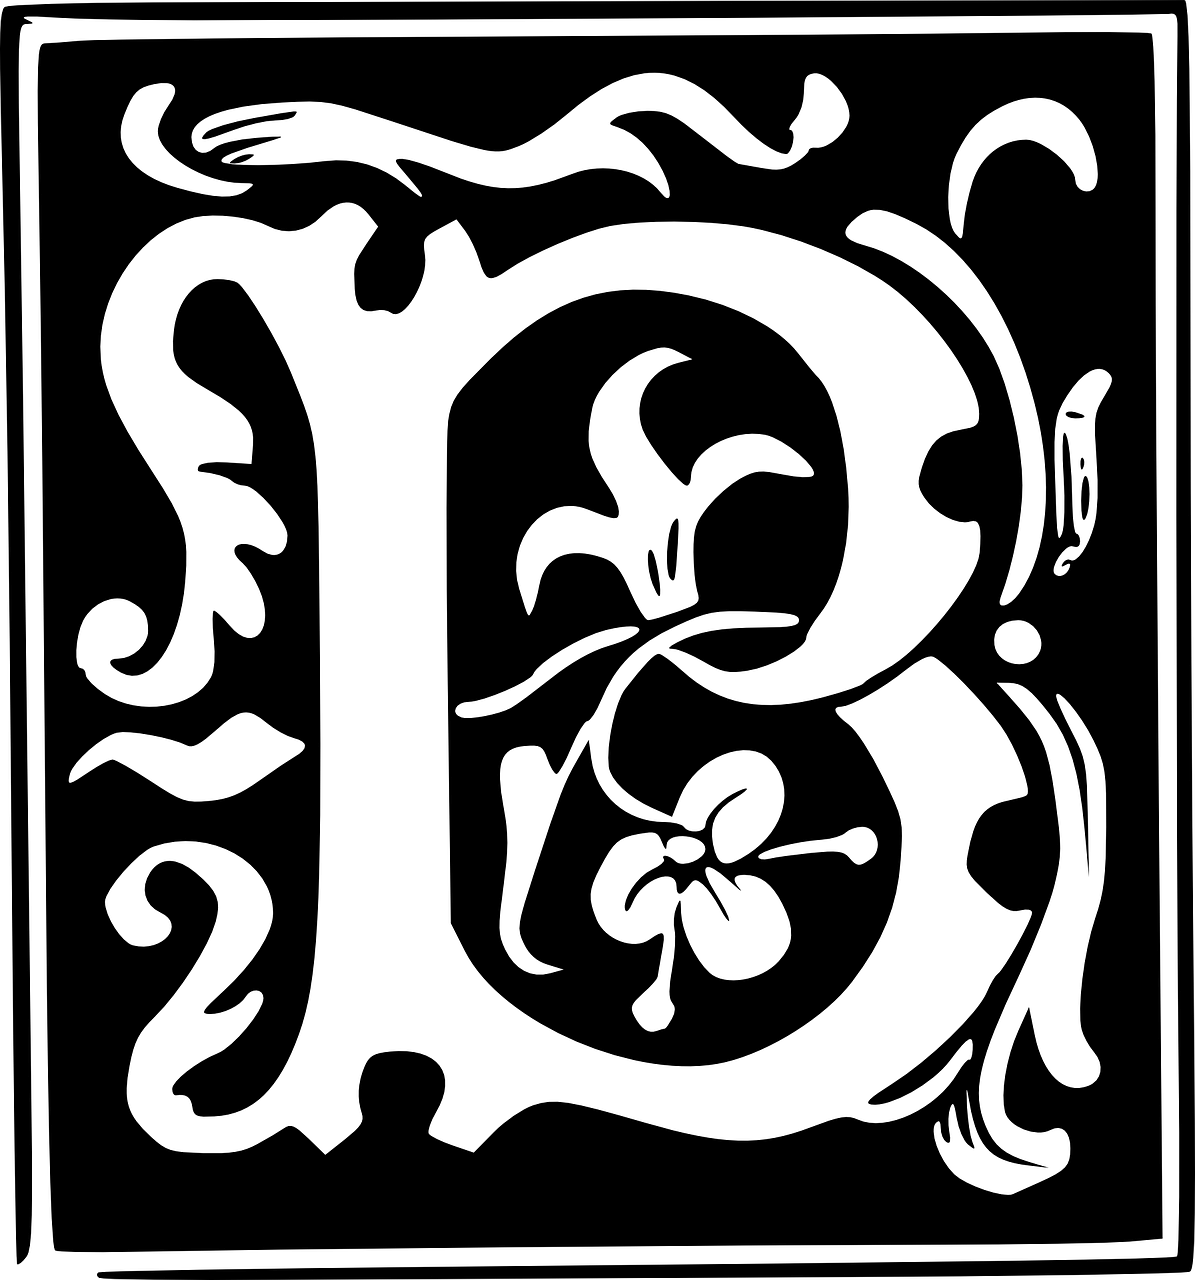
\includegraphics[width=0.85\textwidth]{FancyB.png}
    \caption{Illuminated initial letter B.}
    \label{fig:letterB}
\end{subfigure}
\caption{An example figure containing two subfigures, which may be referenced individually as Figure~\ref{fig:letterA} and Figure~\ref{fig:letterB}, or collectively as Figure~\ref{fig:letters}.}
\label{fig:letters}
\end{figure}

\section{Tables: Standard and Landscape}
\label{sec:tables}

According to NJIT style rules:
\begin{itemize}
\item Table titles are placed \textbf{above} the table.
\item Table titles are formatted in title case and do \textbf{not} end with a period.
\item The table text is single-spaced.
\item Tables are numbered by chapter, like figures.
\item A small table must not be split across pages (GSO).
\item The title appears word for word in the List of Tables.
\item Put the column units in the column header, not in every cell.
\end{itemize}

\subsection{Standard portrait table}
Table~\ref{table:NN_DIFF} illustrates a standard floating table placed in portrait mode, loaded from \texttt{table.tex}.
The table is kept in its own file and pulled in with \verb+\input+. This is optional, but it keeps large tables, or tables generated by a script, out of the chapter text. The \texttt{booktabs} rules used in Table~\ref{table:landscape_sample} (\verb+\toprule+, \verb+\midrule+, \verb+\bottomrule+, and no vertical lines) usually read more cleanly than a full grid.

% !TeX root = main.tex
% Sample table, kept in its own file and included from chapter2.tex with
% % !TeX root = main.tex
% Sample table, kept in its own file and included from chapter2.tex with
% \input{table}. Separate files are optional but handy for large tables or
% tables generated by a script.
%
% GSO rules (the class handles the layout):
% - The title (\caption) goes ABOVE the table, in title case, with no final
%   period. It appears word for word in the List of Tables.
% - Tables are numbered by chapter (Table 2.1).
% - Table text is single-spaced; a small table must not split across pages.
% Refer to every table in the text with \ref{label}.

\begin{table}[htbp]
\centering
\caption{Major Differences Between Neural Networks and Cell Signaling Networks}
\label{table:NN_DIFF}

\begin{tabularx}{\linewidth}{|c|p{0.18\linewidth}|X|X|}
\hline
\textbf{Item} & \textbf{Salient Feature} & \textbf{Neural Networks} & \textbf{Cell Signaling Networks} \\
\hline
(i) & Nodes & All nodes typically identical & Nodes are not all equivalent in performance \\
\hline
(ii) & Structure & Typically layered with feed-forward connections only & Regulatory signals often give rise to feedback connections resulting in cycles \\
\hline
(iii) & Connectivity & Highly connected & More sparsely connected \\
\hline
(iv) & Learning Rule & Connectivity altered to perform a single function (e.g., via a back-propagation algorithm) & Cells must be able to respond to multiple stimuli effectively; changes typically occur via evolutionary processes \\
\hline
\end{tabularx}
\end{table}
. Separate files are optional but handy for large tables or
% tables generated by a script.
%
% GSO rules (the class handles the layout):
% - The title (\caption) goes ABOVE the table, in title case, with no final
%   period. It appears word for word in the List of Tables.
% - Tables are numbered by chapter (Table 2.1).
% - Table text is single-spaced; a small table must not split across pages.
% Refer to every table in the text with \ref{label}.

\begin{table}[htbp]
\centering
\caption{Major Differences Between Neural Networks and Cell Signaling Networks}
\label{table:NN_DIFF}

\begin{tabularx}{\linewidth}{|c|p{0.18\linewidth}|X|X|}
\hline
\textbf{Item} & \textbf{Salient Feature} & \textbf{Neural Networks} & \textbf{Cell Signaling Networks} \\
\hline
(i) & Nodes & All nodes typically identical & Nodes are not all equivalent in performance \\
\hline
(ii) & Structure & Typically layered with feed-forward connections only & Regulatory signals often give rise to feedback connections resulting in cycles \\
\hline
(iii) & Connectivity & Highly connected & More sparsely connected \\
\hline
(iv) & Learning Rule & Connectivity altered to perform a single function (e.g., via a back-propagation algorithm) & Cells must be able to respond to multiple stimuli effectively; changes typically occur via evolutionary processes \\
\hline
\end{tabularx}
\end{table}


\subsection{Landscape orientation for wide tables}
Occasionally, a dissertation table or figure contains too many columns to fit within the standard 6-inch text width of a portrait page. The \texttt{njit\_thesis.cls} class includes built-in landscape capability via \texttt{pdflscape}. The \texttt{landscape} environment rotates the entire page content while keeping headers, footers, and page numbers in their proper orientation, and rotates the PDF page view so that it is easily readable on a screen without neck strain.

The GSO requires that on a landscape page the bottom of the table or figure faces the outer edge of the page, while the page number stays in its normal portrait position. The \texttt{landscape} environment does both.

Table~\ref{table:landscape_sample} on the following page demonstrates a full landscape table.

\begin{landscape}
\begin{table}[htbp]
\centering
\caption{Comparison of Numerical Solvers for Stiff Partial Differential Equations}
\label{table:landscape_sample}
\vspace{6pt}
\begin{tabularx}{\linewidth}{l l c c X}
\toprule
\textbf{Algorithm} & \textbf{Type} & \textbf{Order} & \textbf{Stability} & \textbf{Key Characteristics and Applications} \\
\midrule
Forward Euler & Explicit Runge--Kutta & 1 & Conditionally stable & Simple to implement; severely time-step restricted for stiff parabolic problems. \\
Crank--Nicolson & Implicit Trapezoidal & 2 & A-stable & Unconditionally stable for linear diffusion; exhibits oscillations with discontinuous boundary data. \\
RK4 & Explicit 4-stage RK & 4 & Conditionally stable & High accuracy for non-stiff systems; widely used for hyperbolic conservation laws. \\
BDF2 & Multistep Backward Diff. & 2 & L-stable & Strongly damping high frequencies; standard choice for chemical reaction-diffusion equations. \\
Radau IIA & Implicit Runge--Kutta & 5 & L-stable & Fully implicit; excellent for differential-algebraic equations (DAEs) and stiff Hamiltonian control. \\
\bottomrule
\end{tabularx}
\end{table}
\end{landscape}

\section{Bibliography and Publications Listing}
\label{sec:bibliography}

Bibliographic citations are managed by the modern \texttt{biblatex} package backed by \texttt{biber}. Citations in the text are inserted using the standard \verb+\cite+ command, for example \cite{ALBERTSETAL:1994,FERSHT:1985,FISCHER:1987a,KAUFFMAN:1969,MR1191182,MR1617060}.

Choose a citation style permitted by your program (Table~\ref{tab:phd-styles}) by setting \verb+\mycitestyle+ in \texttt{packages.tex}; do not format references by hand. Whatever the style, the GSO asks that references be consistent in capitalization, punctuation, and format, and that book titles be italicized, not placed in quotation marks. The class sets each reference single-spaced, with a blank line between references.

Most formatting problems in a bibliography come from the \texttt{.bib} file, not from \LaTeX. When you copy entries from Google Scholar or a publisher:
\begin{itemize}
\item Protect capitals that must survive, such as proper names and acronyms, with braces: \verb+title = {Stability of {KdV} solitons in {Hilbert} space}+.
\item Check that author names are separated by \verb+and+, not commas.
\item Write journal names out in full, such as \emph{Journal of Fluid Mechanics} rather than \emph{J.\ Fluid Mech.} Publisher and Google Scholar entries often use abbreviations, so check the \verb+journal+ field of each entry.
\item Check every entry for missing volumes, pages, and years; the style cannot print what isn't there.
\end{itemize}

\subsection{Bibliography styles}

Different fields of study have adopted different bibliography styles, which are conventions for formatting bibliography entries. Table~\ref{tab:phd-styles} lists which styles are permitted by each NJIT Ph.D. program. Some programs permit multiple styles. Table~\ref{tab:citation-styles} shows an example of each style.

\begin{landscape}
\begin{table}[htbp]
\centering
\caption{Ph.D. Programs and Required Citation Styles}
\label{tab:phd-styles}
\begin{tabularx}{\linewidth}{l l}
\toprule
\textbf{Ph.D. Program} & \textbf{Citation Style} \\
\midrule
Applied Physics & ACS, AIP, Harvard \\
Biology & ACS \\
Biomedical Engineering & ACS, AMA, IEEE \\
Business Data Science & APA \\
Chemical Engineering & ACS, AIP, Chicago, Harvard \\
Chemistry & ACS \\
Civil Engineering & ACS, AIP, ASCE, Harvard, IEEE \\
Computer Engineering & IEEE \\
Computer Science & ACM, Chicago, IEEE \\
Data Science (Computing Option) & ACM, IEEE \\
Data Science (Statistics Option) & AMA, Chicago, Harvard, IEEE \\
Electrical Engineering & IEEE \\
Engineering Science & APA, IEEE \\
Environmental Engineering & ACS, AIP, ASCE, Chicago, Harvard \\
Environmental Science & APA \\
Industrial Engineering & APA, IEEE \\
Information Systems & ACM, APA \\
Materials Science and Engineering & ACS, AIP, Chicago, Harvard \\
Mathematical Sciences (Applied Mathematics Option) & AMS \\
Mathematical Sciences (Applied Probability and Statistics Option) & Chicago, Harvard, Vancouver \\
Mechanical Engineering & ACS, AIP, Chicago, Harvard, IEEE \\
Transportation & ACS, AIP, APA, ASCE, Chicago, IEEE, TRB \\
Urban Systems & APA \\
\bottomrule
\end{tabularx}
\end{table}
\end{landscape}

\begin{table}[htbp]
\centering
\caption{Citation Formats for ``PRIMES is in P'' Across Bibliography Styles }
\label{tab:citation-styles}
\begin{tabularx}{\textwidth}{l X}
\toprule
\textbf{Style} & \textbf{Citation} \\
\midrule
ACM & M. Agrawal, N. Kayal, and N. Saxena. 2004. PRIMES is in P. \textit{Annals of Mathematics} 160, 2 (2004), 781--793. \\
\addlinespace
ACS & Agrawal, M.; Kayal, N.; Saxena, N. PRIMES is in P. \textit{Annals of Mathematics} \textbf{2004}, \textit{160} (2), 781--793. \\
\addlinespace
AIP & M. Agrawal, N. Kayal, and N. Saxena, PRIMES is in P, \textit{Annals of Mathematics} \textbf{160} (2), 781--793 (2004). \\
\addlinespace
AMA & Agrawal M, Kayal N, Saxena N. PRIMES is in P. \textit{Annals of Mathematics}. 2004;160(2):781--793. \\
\addlinespace
AMS & M. Agrawal, N. Kayal, and N. Saxena, \textit{PRIMES is in P}, Annals of Mathematics \textbf{160} (2004), no. 2, 781--793. \\
\addlinespace
APA & Agrawal, M., Kayal, N., \& Saxena, N. (2004). PRIMES is in P. \textit{Annals of Mathematics}, \textit{160}(2), 781--793. \\
\addlinespace
ASCE & Agrawal, M., Kayal, N., and Saxena, N. (2004). ``PRIMES is in P.'' \textit{Annals of Mathematics}, 160(2), 781--793. \\
\addlinespace
Chicago & Agrawal, Manindra, Neeraj Kayal, and Nitin Saxena. 2004. ``PRIMES is in P.'' \textit{Annals of Mathematics} 160 (2): 781--793. \\
\addlinespace
Harvard & Agrawal, M., Kayal, N. and Saxena, N., 2004. PRIMES is in P. \textit{Annals of Mathematics}, 160(2), pp.781--793. \\
\addlinespace
IEEE & M. Agrawal, N. Kayal, and N. Saxena, ``PRIMES is in P,'' \textit{Annals of Mathematics}, vol. 160, no. 2, pp. 781--793, 2004. \\
\addlinespace
TRB & Agrawal, M., N. Kayal, and N. Saxena. PRIMES is in P. \textit{Annals of Mathematics}, Vol. 160, No. 2, 2004, pp. 781--793. \\
\addlinespace
Vancouver & Agrawal M, Kayal N, Saxena N. PRIMES is in P. Annals of Mathematics. 2004;160(2):781--793. \\
\bottomrule
\end{tabularx}
\end{table}

\subsection{Managing multiple bibliographies}
A major advantage of \texttt{biblatex} is its ability to produce multiple independent bibliographies. In this template, the Presentations and Publications listing in the Biographical Sketch (page~iv) is populated directly from the \texttt{references.bib} database by filtering for entries that include the tag:
\begin{verbatim}
keywords = {me},
\end{verbatim}
This eliminates the need to maintain two separate citation files.


%%%%%%%%%%%%%%%%%%%%%%%%%%%%%%%%%%%%%%%%%%%%%%%%%%%%%%
%% Appendices
%%%%%%%%%%%%%%%%%%%%%%%%%%%%%%%%%%%%%%%%%%%%%%%%%%%%%%
\appendix

% --- Option A: Single Appendix (Default) ---
% If your dissertation has only ONE appendix, use the \oneappendix{Title}
% command inside appendix.tex. This complies with NJIT's requirement that
% a single appendix has no letter label (not "Appendix A", just "APPENDIX").
% !TeX root = main.tex
% SINGLE APPENDIX. Use this file when the document has exactly ONE appendix
% (it is printed as "APPENDIX", with no letter). Start with
% \oneappendix{Title}. For two or more appendices, use appendixA.tex,
% appendixB.tex, appendixC.tex, ... instead (see main.tex). The sample text
% is shared with appendixA.tex through appendix-rules.tex and appendix-demo.tex.
% Every appendix needs a title and a short introduction before any figures
% or tables (GSO). Numbering restarts at A.1.

\oneappendix{Including an appendix or appendices}
\label{app:appendixA}% same label as appendixA.tex, so references in the chapters work either way

% !TEX root = main.tex
% Shared text: the GSO rules for appendices. Included with \input from both
% appendix.tex (single appendix) and appendixA.tex (several appendices), so
% the wording lives in one place. Delete this file and its \input lines
% when you write your own appendices.

An appendix holds material that supports the dissertation but that a reader does not need in order to follow the argument. A useful test: if a reader skipped the appendix, would the chapters still make sense and still support their conclusions? If not, the material belongs in a chapter.

\textbf{Keep in the chapters} everything a reader needs to follow and evaluate the work:
\begin{itemize}
\item the research questions, the methods, and the main results;
\item the figures and tables that present those results;
\item the key steps of the central proofs and derivations.
\end{itemize}

\textbf{Move to an appendix} material that is long, routine, or of interest mainly to a specialist checking the details:
\begin{itemize}
\item long or routine proofs and derivations, once the chapter has stated the result;
\item full data tables, when the chapter shows a summary;
\item additional figures that repeat a result for other parameters or cases;
\item survey instruments, interview protocols, and consent forms;
\item long source code or pseudocode;
\item details of experimental setups, calibrations, and numerical parameters.
\end{itemize}

Refer to every appendix from the chapter where its material is relevant, for example ``The full proof is given in Appendix~B.'' Material that no chapter refers to probably does not belong in the dissertation at all. Large data sets and complete software packages usually do not belong in an appendix either; deposit them in a public repository and cite them, or ask the GSO how to submit supplementary files.

NJIT enforces a strict rule regarding the titling and numbering of appendices:
\begin{itemize}
\item If your dissertation has only a \textbf{single appendix}, it must be titled \textbf{APPENDIX} (without any letter label such as "A"), followed by the appendix title.
\item If your dissertation contains \textbf{two or more appendices}, they must be numbered sequentially as \textbf{APPENDIX A}, \textbf{APPENDIX B}, etc.
\end{itemize}

You should not try to format this manually. Instead:
\begin{itemize}
\item If you have \textbf{one} appendix, use \texttt{appendix.tex} and begin it with the command \verb+\oneappendix{Your Title}+. The heading prints as APPENDIX followed by your title in capitals.
\item If you have \textbf{two or more}, switch to the multi-appendix lines in \texttt{main.tex} and begin each file with \verb+\chapter{Your Title}+. They are lettered A, B, \ldots\ automatically.
\end{itemize}

Every appendix needs a title and a brief introductory description before any equations, figures, or tables (GSO). Appendix pages are numbered continuously with the chapters, and equations, figures, and tables in an appendix are numbered with the appendix letter, starting again at 1 (A.1, B.1, \ldots).


This template uses a single appendix, so its equations, figures, and tables are numbered A.1, A.2, and so on, as below.

% !TeX root = main.tex
% Shared sample: demonstrates numbered equations, figures, and a table inside
% an appendix. Included with \input from appendix.tex (single appendix) and
% appendixA.tex (lettered appendices); only one of those is compiled at a
% time, so each label is defined once. Delete this file and its \input lines
% when you write your own appendices.

\section{Equations and Figures in Appendices}

Equations inside the appendix are numbered with an appendix prefix:
\begin{align}
\label{eq:app1}
\nabla^2 \phi - \frac{1}{c^2}\frac{\partial^2 \phi}{\partial t^2} &= 0, \\
\label{eq:app2}
\oint_{\partial \Omega} \mathbf{F} \cdot d\mathbf{S} &= \iiint_{\Omega} (\nabla \cdot \mathbf{F})\, dV.
\end{align}
Cross-references like Equation~\eqref{eq:app1} and Equation~\eqref{eq:app2} resolve cleanly.

Figures placed within the appendix also receive appropriate appendix numbering, as shown in Figure~\ref{fig:app_cube1} and Figure~\ref{fig:app_cube2}.

\begin{figure}[htbp]
\centering

\includegraphics[width=2.5in]{msgcube}
\caption{First appendix demonstration figure.}
\label{fig:app_cube1}
\end{figure}

\begin{figure}[htbp]
\centering

\includegraphics[width=2.5in]{msgcube}
\caption{Second appendix demonstration figure.}
\label{fig:app_cube2}
\end{figure}

\clearpage
\section{Tables in an appendix}

Here is an example of a table in an appendix showing how you might typeset a table of websites you consulted in your thesis. 
Table~\ref{table:WEBSITES} lists common bioinformatics and signaling databases, formatted with automatic line wrapping for URLs using the \texttt{xurl} package.

\begin{table}[htbp]
\centering
\caption{Key Online Databases for Cell Signaling and Molecular Biology}
\label{table:WEBSITES}
\begin{tabularx}{\linewidth}{|c|p{0.32\linewidth}|X|}
\hline
\textbf{\#} & \textbf{Resource / URL} & \textbf{Description} \\
\hline
1 & \url{http://vlib.org/Science/Cell_Biology} & Virtual Library for Cell Biology with curated signal transduction pathways. \\
\hline
2 & \url{http://www.grt.kyushu-u.ac.jp/spad/} & Signaling Pathway Database containing curated pathway diagrams. \\
\hline
3 & \url{http://geo.nihs.go.jp/csndb/} & Cell Signaling Networks Database (CSNDB) \cite{CSND:1999}. \\
\hline
4 & \url{http://www.sdsc.edu/kinases/} & Protein Kinase Resource (PKR) for protein kinase structural data \cite{PKR:1997}. \\
\hline
5 & \url{http://www.expasy.ch/sprot/} & SWISS-PROT annotated protein sequence database \cite{BAIROCH:2000}. \\
\hline
6 & \url{http://www.expasy.ch/prosite/} & PROSITE database of protein families and functional domains \cite{HOFMANN:1999}. \\
\hline
7 & \url{http://www.rcsb.org/pdb/} & Protein Data Bank (PDB) for 3D macromolecular structures \cite{BERMAN:2000}. \\
\hline
\end{tabularx}
\end{table}



% --- Option B: Multiple Appendices ---
% If your dissertation has TWO OR MORE appendices, comment out the line above
% and uncomment the lines below. Each file should start with \chapter{Title}.
%% !TEX root = main.tex
% APPENDIX A (one of several). Use appendixA.tex, appendixB.tex, ... when the
% document has TWO OR MORE appendices (they are lettered A, B, ...).
% Start each file with \chapter{Title}; \appendix in main.tex switches
% chapters to appendix lettering. Every appendix needs a title and a short
% introduction before any figures or tables (GSO).
% The sample text is shared with appendix.tex through appendix-rules.tex and
% appendix-demo.tex.

\chapter{Including an appendix or appendices}
\label{app:appendixA}

% !TEX root = main.tex
% Shared text: the GSO rules for appendices. Included with \input from both
% appendix.tex (single appendix) and appendixA.tex (several appendices), so
% the wording lives in one place. Delete this file and its \input lines
% when you write your own appendices.

An appendix holds material that supports the dissertation but that a reader does not need in order to follow the argument. A useful test: if a reader skipped the appendix, would the chapters still make sense and still support their conclusions? If not, the material belongs in a chapter.

\textbf{Keep in the chapters} everything a reader needs to follow and evaluate the work:
\begin{itemize}
\item the research questions, the methods, and the main results;
\item the figures and tables that present those results;
\item the key steps of the central proofs and derivations.
\end{itemize}

\textbf{Move to an appendix} material that is long, routine, or of interest mainly to a specialist checking the details:
\begin{itemize}
\item long or routine proofs and derivations, once the chapter has stated the result;
\item full data tables, when the chapter shows a summary;
\item additional figures that repeat a result for other parameters or cases;
\item survey instruments, interview protocols, and consent forms;
\item long source code or pseudocode;
\item details of experimental setups, calibrations, and numerical parameters.
\end{itemize}

Refer to every appendix from the chapter where its material is relevant, for example ``The full proof is given in Appendix~B.'' Material that no chapter refers to probably does not belong in the dissertation at all. Large data sets and complete software packages usually do not belong in an appendix either; deposit them in a public repository and cite them, or ask the GSO how to submit supplementary files.

NJIT enforces a strict rule regarding the titling and numbering of appendices:
\begin{itemize}
\item If your dissertation has only a \textbf{single appendix}, it must be titled \textbf{APPENDIX} (without any letter label such as "A"), followed by the appendix title.
\item If your dissertation contains \textbf{two or more appendices}, they must be numbered sequentially as \textbf{APPENDIX A}, \textbf{APPENDIX B}, etc.
\end{itemize}

You should not try to format this manually. Instead:
\begin{itemize}
\item If you have \textbf{one} appendix, use \texttt{appendix.tex} and begin it with the command \verb+\oneappendix{Your Title}+. The heading prints as APPENDIX followed by your title in capitals.
\item If you have \textbf{two or more}, switch to the multi-appendix lines in \texttt{main.tex} and begin each file with \verb+\chapter{Your Title}+. They are lettered A, B, \ldots\ automatically.
\end{itemize}

Every appendix needs a title and a brief introductory description before any equations, figures, or tables (GSO). Appendix pages are numbered continuously with the chapters, and equations, figures, and tables in an appendix are numbered with the appendix letter, starting again at 1 (A.1, B.1, \ldots).


This sample has five appendices, so they are lettered: this is \textbf{APPENDIX A}, followed by \cref{app:citestyles}, which collects guides to the citation styles, \cref{app:packages}, which describes the packages the template loads, \cref{app:filetree}, which lists the template's files, and \cref{app:supplementary}, which lists supplementary files. The class file prints the letters in the headings and the Table of Contents and prefixes equations, theorems, figures, and tables with the letter, as the examples below show. To switch to a single, unlettered appendix, follow the instructions at the end of \texttt{main.tex}.

% !TeX root = main.tex
% Shared sample: demonstrates numbered equations, figures, and a table inside
% an appendix. Included with \input from appendix.tex (single appendix) and
% appendixA.tex (lettered appendices); only one of those is compiled at a
% time, so each label is defined once. Delete this file and its \input lines
% when you write your own appendices.

\section{Equations and Figures in Appendices}

Equations inside the appendix are numbered with an appendix prefix:
\begin{align}
\label{eq:app1}
\nabla^2 \phi - \frac{1}{c^2}\frac{\partial^2 \phi}{\partial t^2} &= 0, \\
\label{eq:app2}
\oint_{\partial \Omega} \mathbf{F} \cdot d\mathbf{S} &= \iiint_{\Omega} (\nabla \cdot \mathbf{F})\, dV.
\end{align}
Cross-references like Equation~\eqref{eq:app1} and Equation~\eqref{eq:app2} resolve cleanly.

Figures placed within the appendix also receive appropriate appendix numbering, as shown in Figure~\ref{fig:app_cube1} and Figure~\ref{fig:app_cube2}.

\begin{figure}[htbp]
\centering

\includegraphics[width=2.5in]{msgcube}
\caption{First appendix demonstration figure.}
\label{fig:app_cube1}
\end{figure}

\begin{figure}[htbp]
\centering

\includegraphics[width=2.5in]{msgcube}
\caption{Second appendix demonstration figure.}
\label{fig:app_cube2}
\end{figure}

\clearpage
\section{Tables in an appendix}

Here is an example of a table in an appendix showing how you might typeset a table of websites you consulted in your thesis. 
Table~\ref{table:WEBSITES} lists common bioinformatics and signaling databases, formatted with automatic line wrapping for URLs using the \texttt{xurl} package.

\begin{table}[htbp]
\centering
\caption{Key Online Databases for Cell Signaling and Molecular Biology}
\label{table:WEBSITES}
\begin{tabularx}{\linewidth}{|c|p{0.32\linewidth}|X|}
\hline
\textbf{\#} & \textbf{Resource / URL} & \textbf{Description} \\
\hline
1 & \url{http://vlib.org/Science/Cell_Biology} & Virtual Library for Cell Biology with curated signal transduction pathways. \\
\hline
2 & \url{http://www.grt.kyushu-u.ac.jp/spad/} & Signaling Pathway Database containing curated pathway diagrams. \\
\hline
3 & \url{http://geo.nihs.go.jp/csndb/} & Cell Signaling Networks Database (CSNDB) \cite{CSND:1999}. \\
\hline
4 & \url{http://www.sdsc.edu/kinases/} & Protein Kinase Resource (PKR) for protein kinase structural data \cite{PKR:1997}. \\
\hline
5 & \url{http://www.expasy.ch/sprot/} & SWISS-PROT annotated protein sequence database \cite{BAIROCH:2000}. \\
\hline
6 & \url{http://www.expasy.ch/prosite/} & PROSITE database of protein families and functional domains \cite{HOFMANN:1999}. \\
\hline
7 & \url{http://www.rcsb.org/pdb/} & Protein Data Bank (PDB) for 3D macromolecular structures \cite{BERMAN:2000}. \\
\hline
\end{tabularx}
\end{table}


%% !TeX root = main.tex

\chapter{Supplementary Data and Computational Parameters}
\label{app:data}

This appendix illustrates a second appendix (\textbf{APPENDIX B}) when multiple appendices are present.

\section{Computational Grid Settings}
\label{sec:appB_grid}

Table~\ref{table:appB_params} summarizes the numerical grid discretization and tolerance parameters employed in numerical simulations throughout this work.

\begin{table}[htbp]
\centering
\caption{Numerical Simulation Grid and Solver Parameters}
\label{table:appB_params}
\vspace{6pt}
\begin{tabularx}{0.85\linewidth}{|l|c|X|}
\hline
\textbf{Parameter} & \textbf{Value} & \textbf{Physical Meaning / Role} \\
\hline
Spatial domain $L$ & $100.0$ & Total length of periodic spatial domain \\
\hline
Grid points $N_x$ & $1024$ & Number of spatial Fourier discretization points \\
\hline
Time step $\Delta t$ & $10^{-3}$ & Integration time step \\
\hline
Absolute tolerance & $10^{-10}$ & Local error tolerance for adaptive time stepping \\
\hline
Relative tolerance & $10^{-8}$ & Relative error tolerance \\
\hline
\end{tabularx}
\end{table}

Euler's identity provides the celebrated benchmark relation:
\begin{equation}
\label{eq:appB_euler}
e^{i\pi} + 1 = 0.
\end{equation}
Notice that in the Table of Contents and in Equation~\eqref{eq:appB_euler}, all references are prefixed with the letter \textbf{B}.

%%%%%%%%%%%%%%%%%%%%%%%%%%%%%%%%%%%%%%%%%%%%%%%%%%%%%%
%% Bibliography / References
%%%%%%%%%%%%%%%%%%%%%%%%%%%%%%%%%%%%%%%%%%%%%%%%%%%%%%
\clearpage
\addcontentsline{toc}{chapter}{REFERENCES}
\printbibliography[title={References}]

\end{document}